%%%%%%%% ICML 2023 EXAMPLE LATEX SUBMISSION FILE %%%%%%%%%%%%%%%%%

\documentclass{article}

% Recommended, but optional, packages for figures and better typesetting:
\usepackage{microtype}
\usepackage{graphicx}
\usepackage{subfigure}
\usepackage{booktabs} % for professional tables

% hyperref makes hyperlinks in the resulting PDF.
% If your build breaks (sometimes temporarily if a hyperlink spans a page)
% please comment out the following usepackage line and replace
% \usepackage{icml2023} with \usepackage[nohyperref]{icml2023} above.
\usepackage{hyperref}


% Attempt to make hyperref and algorithmic work together better:
\newcommand{\theHalgorithm}{\arabic{algorithm}}

% Use the following line for the initial blind version submitted for review:
%\usepackage{icml2023}

% If accepted, instead use the following line for the camera-ready submission:
 \usepackage[accepted]{icml2023}

% For theorems and such
\usepackage{amsmath}
\usepackage{amssymb}
\usepackage{mathtools}
\usepackage{amsthm}

% if you use cleveref..
\usepackage[capitalize,noabbrev]{cleveref}

%%%%%%%%%%%%%%%%%%%%%%%%%%%%%%%%
% THEOREMS
%%%%%%%%%%%%%%%%%%%%%%%%%%%%%%%%
\theoremstyle{plain}
\newtheorem{theorem}{Theorem}[section]
\newtheorem{proposition}[theorem]{Proposition}
\newtheorem{lemma}[theorem]{Lemma}
\newtheorem{corollary}[theorem]{Corollary}
\theoremstyle{definition}
\newtheorem{definition}[theorem]{Definition}
\newtheorem{assumption}[theorem]{Assumption}
\theoremstyle{remark}
\newtheorem{remark}[theorem]{Remark}

% Todonotes is useful during development; simply uncomment the next line
%    and comment out the line below the next line to turn off comments
%\usepackage[disable,textsize=tiny]{todonotes}
\usepackage[textsize=tiny]{todonotes}


% The \icmltitle you define below is probably too long as a header.
% Therefore, a short form for the running title is supplied here:
\icmltitlerunning{Idiolect: A Reconfigurable Voice Coding Assistant}

\begin{document}

\twocolumn[
\icmltitle{Idiolect: A Reconfigurable Voice Coding Assistant}

%\icmlsetsymbol{equal}{*}

\begin{icmlauthorlist}
\icmlauthor{Breandan Considine}{yyy}
\icmlauthor{Nicholas Albion}{comp}
\icmlauthor{Xujie Si}{sch}
\end{icmlauthorlist}

\icmlaffiliation{yyy}{McGill University}
\icmlaffiliation{comp}{Independent Researcher}
\icmlaffiliation{sch}{University of Toronto}

\icmlcorrespondingauthor{Breandan Considine}{bre@ndan.co}

% You may provide any keywords that you
% find helpful for describing your paper; these are used to populate
% the "keywords" metadata in the PDF but will not be shown in the document
\icmlkeywords{Machine Learning, ICML}

\vskip 0.3in
]

% this must go after the closing bracket ] following \twocolumn[ ...

% This command actually creates the footnote in the first column
% listing the affiliations and the copyright notice.
% The command takes one argument, which is text to display at the start of the footnote.
% The \icmlEqualContribution command is standard text for equal contribution.
% Remove it (just {}) if you do not need this facility.

%\printAffiliationsAndNotice{}  % leave blank if no need to mention equal contribution
%\printAffiliationsAndNotice{} % otherwise use the standard text.

\begin{abstract}
    Idiolect\footnote{\url{https://youtu.be/R4TDx8GAa-c}} is an open source~\footnote{\url{https://github.com/OpenASR/idiolect}} tool for voice coding and a novel approach to building chatbots that lets users define custom commands and grammars on-the-fly. Unlike traditional chatbots, Idiolect does not impersonate an obedient assistant, but instead offers a highly-configurable interface for automating repetitive programming tasks. Featuring advanced support for error correction and audio-visual feedback, Idiolect promises to enhance the usability and accessibility of manual developer tools by offering an alternate input method for keyboardless programming. The following paper explores the mechanics of voice programming in Idiolect, and sheds light into the challenges faced and insights gained during its development.
\end{abstract}

\section{Introduction}

Humans are able to quickly learn new words and phrases, and apply them in a variety of contexts. Traditional chatbots, however, are often limited to a set of static commands. This creates a frustrating experience for users, who struggle to express their intent, as well as bot developers, who must anticipate user intent and make new capabilities discoverable. This rigidity is a common source of misalignment between user intent, author expectations and bot capabilities.

One direction to address this problem is to improve intent recognition, however, in this paper, we explore the design and implementation of a reconfigurable chatbot for programmers. Idiolect is a programmable voice assistant designed for developers working in an integrated development environment (IDE) or a general-purpose programming context, with a focus on usability, configurability and accessibility.

Idiolect provides a default vocabulary of phrases, but does not impose them upon end-users. Instead, users may configure custom voice commands on-the-fly, which are incorporated into the vocabulary instantly. By shifting the burden of adaptation from the user to the system, this frees our users to express their intent in a more natural manner.

Primarily, Idiolect observes the following design principles: be (1) natural to use, (2) easy to configure, (3) as unobtrusive as possible. We believe that these principles are important for a system intended to be used by developers, who are busy people and quite capable of configuring the system themselves. We also support developers with visual and motor impairments, who may have difficulty typing, or prefer to use a voice interface for the sake of convenience.

\section{Background}

%Mary Shaw, during her 2022 SPLASH keynote~\cite{shaw2022myths} called for programming languages to address the needs of ``vernacular developers''. Jin Guo has also talked about the need for programming in ``ordinary people's language''. We take their proposals quite literally to mean that computers should be able to interpret spoken programs, and not just written ones.

Early attempts to build keyboardless programming systems can be traced back at least two decades to \citet{leopold1997keyboardless}, later revisited by \citet{arnold2000programming}, \citet{begel2005spoken} and others. These systems allow users to write code by speaking into a microphone, however early voice programming systems were limited by a small vocabularies. Another stream of work from \citet{chkroun2019lia} targets teachable voice user interfaces, but unlike our work, do not consider IDE integration or configuration. It also predates many of the recent breakthroughs on large language modeling, which we consider a transformative enabling technology for the adoption of voice programming.

A few commercial solutions such as GitHub Copilot Voice, Serande.ai, and Talon Voice have been developed, but there is comparatively little supporting research on spoken programming. Spoken programs are closely related to natural language programming, an idea once scorned~\cite{dijkstra1979foolishness}, but now becoming increasingly plausible, thanks to the emergence of large language models. \citet{shaw2022myths} calls for new programming languages to address the needs of ``vernacular developers''. As noted by \citet{pandey2022accessibility}, most IDEs are inaccessible to screenreaders and other assistive technologies used by the visually impaired, thus motivating the need for more context-aware voice programming tools.

\section{Architecture}

Today, automatic speech recognition (ASR), the translation of an audio waveform containing speech to text, is essentially a solved problem -- one of the many pretrained ASR models would work well enough for our purposes. By default, Idiolect integrates with Vosk, a state-of-the-art deep speech system with realtime models for offline recognition. This allows us to provide a high-quality speech recognition experience without requiring users to share personal data.

%Users may optionally configure a built-in TTS voice from the host operating system and a cloud-based speech recognition or synthesis service, with the caveat that web speech requires uninterrupted internet connectivity and introduces an additional 300-500ms of overhead latency depending on the user's proximity to the datacenter and other load factors.

\begin{figure}[t]
    \centering
    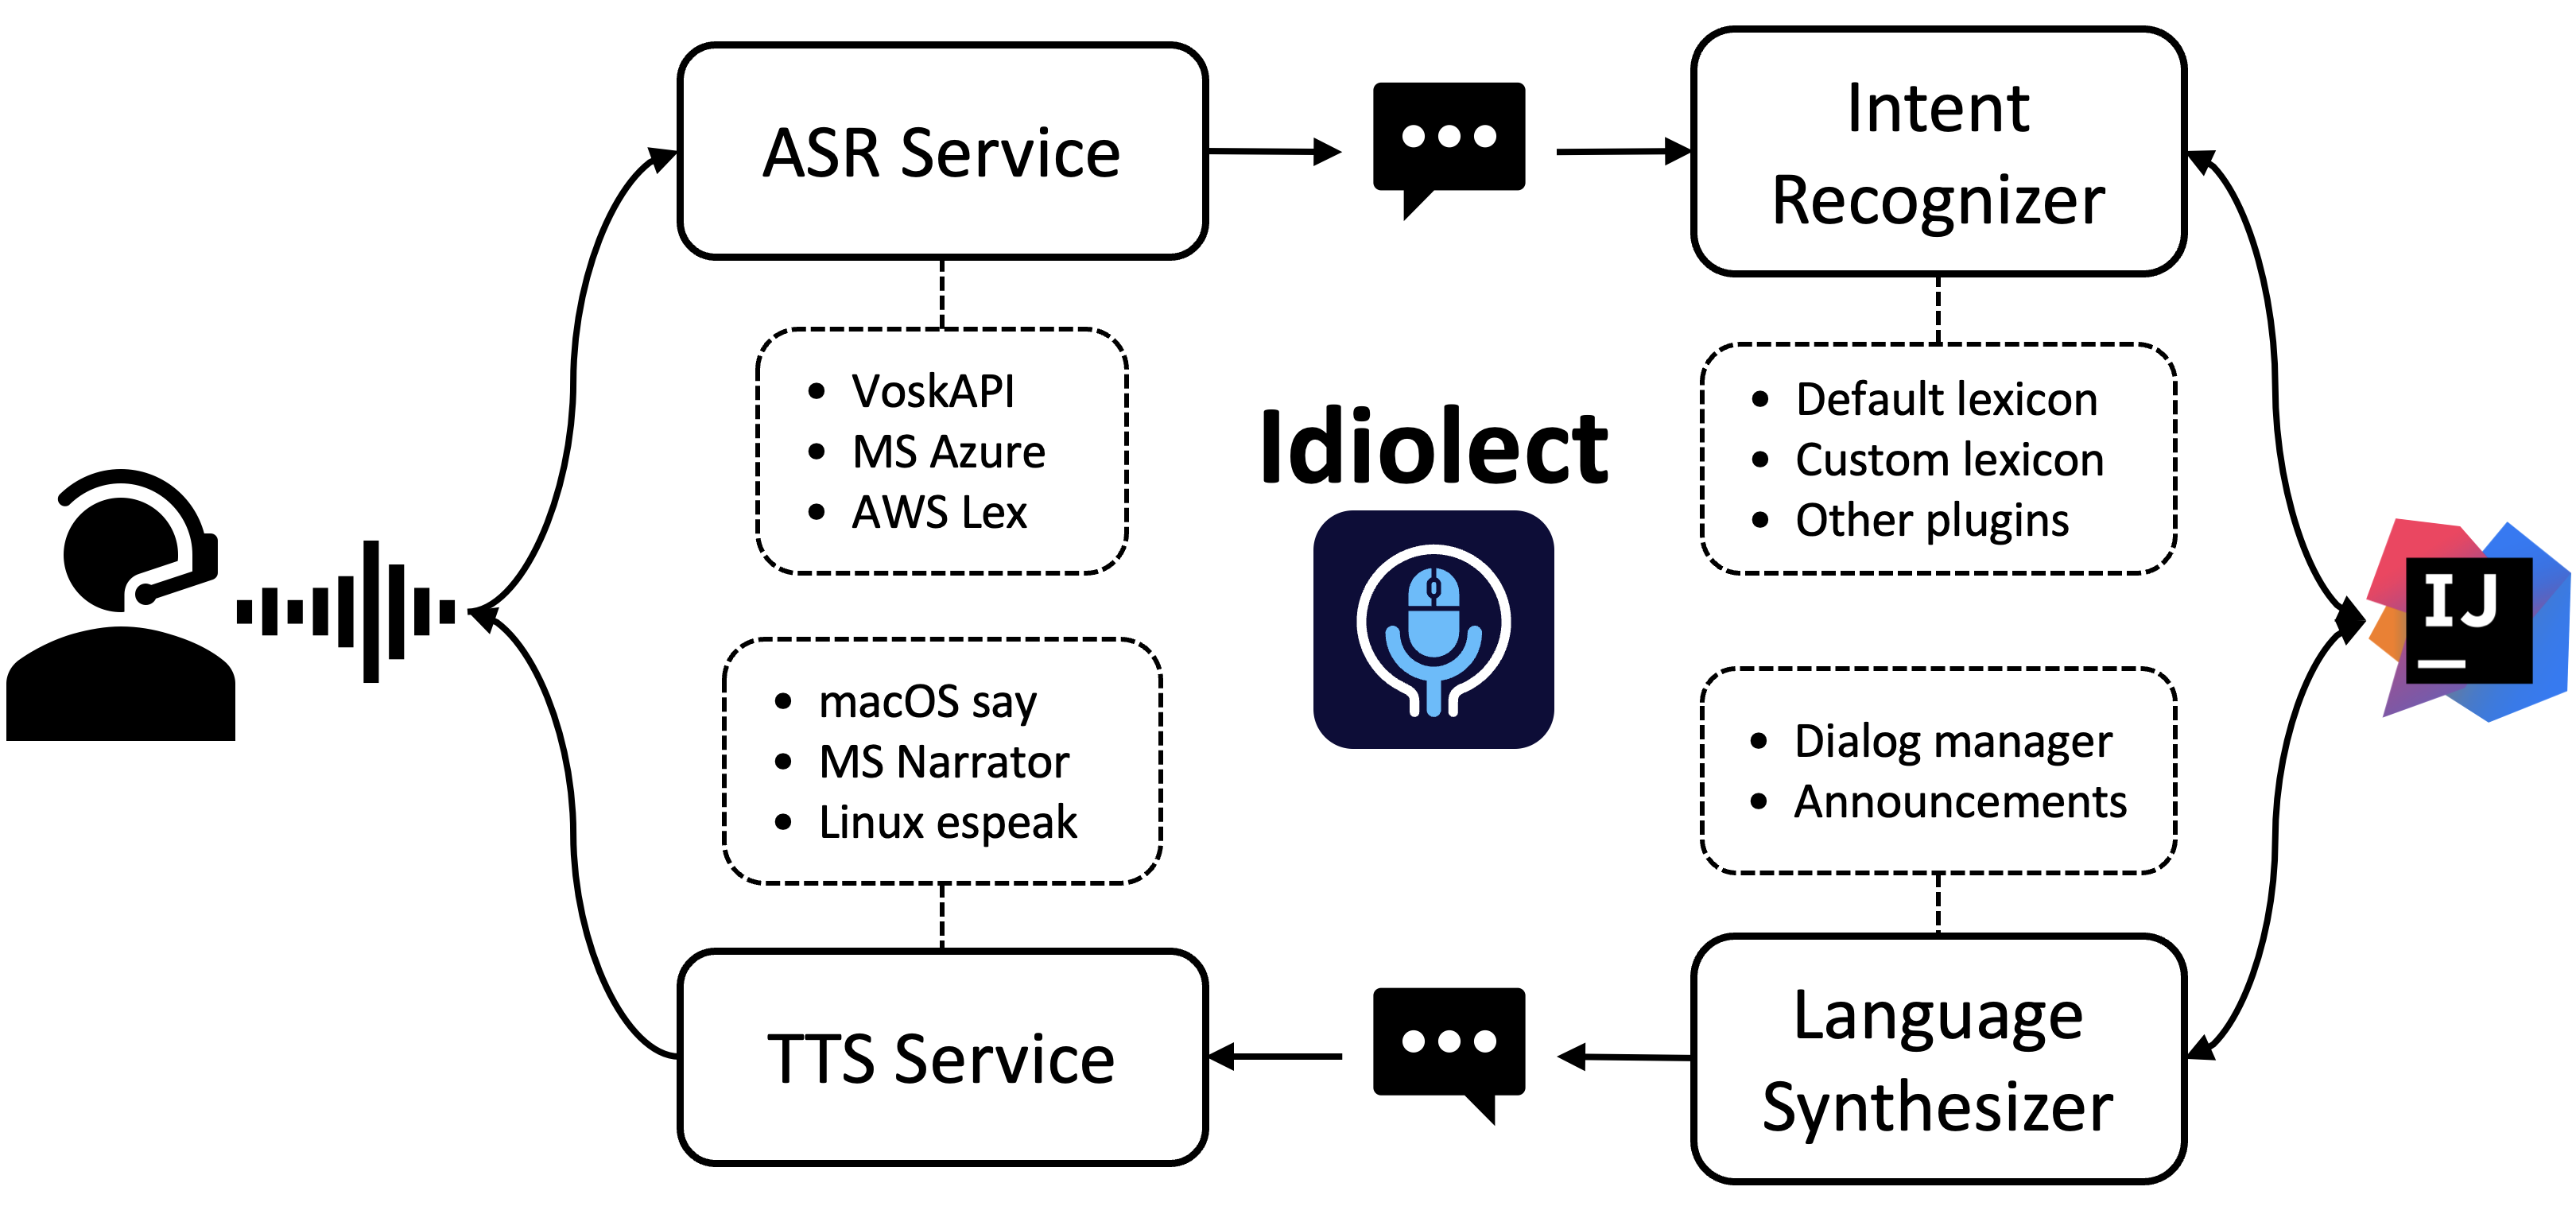
\includegraphics[width=0.9\linewidth]{architecture.png}
    \caption{Idiolect has four major components: a speech and intent recognizer, language synthesizer, and TTS service.}
    \label{fig:architectural_overview}
\end{figure}

Once a spoken utterance is decoded as text, Idiolect must determine the relevant actions and entities needed to fulfill the command. Furthermore, it may need to consider the IDE context, i.e., the current editor state and command history, to resolve potentially ambiguous commands. For example, the phrase, ``open plugin menu'' could refer to multiple different menus, depending on when and how it was invoked.

The IntelliJ Platform has over $10^3$ possible actions. These actions are bound to keyboard shortcuts, menu items, and toolbar buttons. The user can also bind a voice command directly to an action, presuming the user already knows the action's identifier. Idiolect's default grammar was manually curated from the IDE action list, using the CamelCase identifier to generate a suitable description for intent recognition.

Idiolect dispatches utterances to a series of recognizers using a turn-based priority queue, in which each recognizer is given a single turn to match or pass on each utterance. Once a command is recognized, the command is consumed and dispatched to no subsequent recognizer thereafter, which prevents a single command from triggering multiple actions.

\section{Barriers and Pathways to Usability}\label{sec:usability}

We have observed some common usability challenges arise during the development of Idiolect and will now discuss some of those obstacles and our efforts to overcome them.

\subsection{User Onboarding}

Several users reported confusion when first installing our plugin. To address this issue, we added a wizard that guides users through installation. Upon first installing the plugin, a user is greeted and prompted to download the Vosk model for recognizing their preferred natural language, configure the properties file, and bind a few voice commands.

\subsection{Plugin Observability}

Recognition failure is a common issue, often caused by transcription errors in the ASR model, due to, e.g., noise in the audio signal, stopwords, or mistranscription. To address this issue, we added visual cues displaying the phrase transcribed, the action triggered upon intent recognition, and the raw audio waveform. These cues allow users to more easily diagnose and prevent recognition errors from reoccurring.

\subsection{API Extensibility}

Idiolect tries to anticipate users' actions and expose default action bindings, however certain functionality is often best left implemented by downstream developers, who are better-equipped to understand their users' needs. In addition to end-user configurability, Idiolect is designed to be extensible by other IntelliJ Platform plugins, for defining recognition handlers and custom actions. We offer a simple message-passing API for plugins to communicate with Idiolect, and a DSL for defining custom commands and grammars.

\subsection{Error Recovery}\label{sec:error}

Another common usability barrier is when transcription is accurate, but the utterance does not correspond to an actionable command, possibly due to stopwords, verbal fillers or extraneous words which cannot be directly parsed. To recover from recognition failure, we adapt \citet{considine2022tidyparse}, which supports the recognition and parsing of context-free and mildly context-sensitive grammars, and computing language edit distance. This allows Idiolect to recover from minor recognition errors by searching for the closest matching command in a user-defined grammar.

%VoskAPI is also capable of returning a list of alternate utterances alongside a confidence score for each, which can be used to determine if any recognized utterance is sufficiently close to an actionable command in the Idiolect grammar.

%\section{Evaluation}
%
%We conducted a preliminary experiment to evaluate recognition performance on synthetic speech. Using a set of English TTS voices (both male and female) included in macOS Ventura 13.1 with IntelliJ IDEA 2023.1, VoskAPI 0.3.45 and Idiolect 1.3.3, we synthesized 100 utterances from the predefined command list using the \texttt{say} command, then transcoded a 16000 Hz PCM signed 16-bit little-endian audio recording using \texttt{ffmpeg}, and finally transcribe the audio using VoskAPI to simulate a user-generated utterance. We report the average word error rate (WER) of three ASR models trained on US English speakers: \texttt{vosk-model-en-us-0.22} (0.63), \texttt{vosk-model-en-us-0.22-lgraph} (0.66) and \texttt{vosk-model-small-en-us-0.15} (0.73). Results on a per-voice and per-model basis are shown in  Fig.~\ref{fig:fig1} below.
%
%\begin{figure}[ht!]
%    \centering
%    \begin{sidewaystable}
%        \resizebox{.48\textwidth}{!}{% <------ Don't forget this %
%            \begin{tabular}{c*{8}{R}}
%                & \multicolumn{1}{c}{Eddy} & \multicolumn{1}{c}{Flo} & \multicolumn{1}{c}{Fred} &
%                \multicolumn{1}{c}{Reed} & \multicolumn{1}{c}{Rocko} &
%                \multicolumn{1}{c}{Samantha} & \multicolumn{1}{c}{Sandy} &
%                \multicolumn{1}{c}{Shelly} \\[1em]
%                \ldots\texttt{-en-us-0.22}       \hspace{10pt} & 0.581 & 0.635 & 0.888 & 0.627 & 0.981 & 0.293 & 0.492 & 0.528 \\
%                \ldots\texttt{-en-us-0.22-lgraph}\hspace{10pt} & 0.631 & 0.659 & 0.877 & 0.672 & 0.977 & 0.346 & 0.544 & 0.569 \\
%                \ldots\texttt{-small-en-us-0.22} \hspace{10pt} & 0.793 & 0.736 & 0.905 & 0.760 & 0.998 & 0.271 & 0.725 & 0.661 \\
%            \end{tabular}
%        }
%    \end{sidewaystable}
%    \caption{WER for synthetic ASR using 100 commands from the default lexicon across three US English models and seven TTS voices (lower is better).}
%    \label{fig:fig1}
%\end{figure}
%
%WER is a common metric for evaluating ASR performance. We use it to estimate overall intelligibility, but acknowledge it does not account for the quality or diversity of natural speech.
%
%Two primary trends are evident. First, model size has a weak, but observable effect on recognition performance, consistent with prior work on large-vocabulary continuous speech recognition. Based on plentiful evidence in the scaling literature~\cite{droppo2021scaling}, we expect this trend to hold for larger models across natural languages. Out of the three models we tested, \texttt{vosk-model-small-en-us-0.22} exhibits the lowest average WER across all voices. Second, we note the presence of gender bias in the MacOS/Vosk TTS/ASR pipeline. Despite the apparent intelligibility of both sets of voices, WER is substantially lower on female voices (Flo, et al.) than their corresponding male counterparts (Eddy, et al.). The cause of this discrepancy is unclear, but merits further investigation.

\section{Conclusion}

On one end of the design spectrum are embedded domain specific languages (eDSLs). These systems can be powerful, but require a high upfront investment from the user. On the other end are static languages, which can be challenging to maintain and extend. In the middle of this language design spectrum are \textit{idiolects}, which give users the freedom to create, share and reconfigure conversational domain-specific languages for their own idiomatic needs. By targeting developers, who are typically comfortable with configuration languages, commands with more complex semantics can be expressed programmatically, then invoked on-the-fly.

We believe the intersection between conversational agents, vernacular programming languages and programmable voice assistants to be fertile ground, and one relatively unexplored in the language design space. Hopefully, our small contribution inspires others to explore and take similar steps towards making programming more natural and accessible.

\nocite{langley00}

\bibliography{teach}
\bibliographystyle{icml2023}

\end{document}
